\chapter{はじめに}
\section{背景}
こんな感じで文章はファイルをチャプターごとに管理していったほうがいいです

図の参照に関しては「main.tex」を基準にどこにあるかを記述すること(間違えるとコンパイルエラーが出ます)
以下のようにすると\figref{fig::fig_path}が出力されます.

\begin{verbatim}
    \begin{figure}[htb]
        \centering
        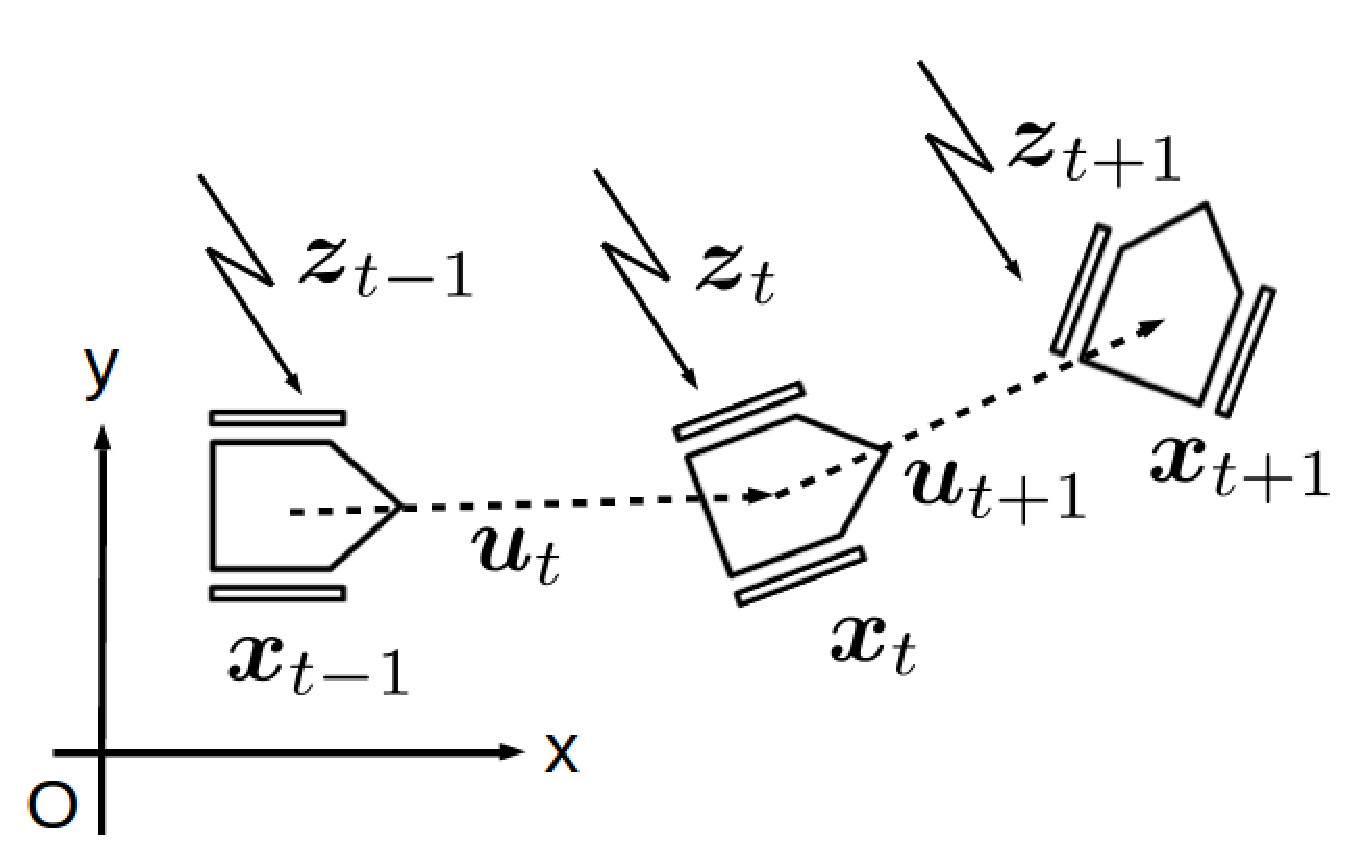
\includegraphics[width = 8cm]{./fig/symbol.eps}
        \caption{example of figure path}
        \label{fig::fig_path}
    \end{figure}
\end{verbatim}


\begin{figure}[htb]
    \centering
    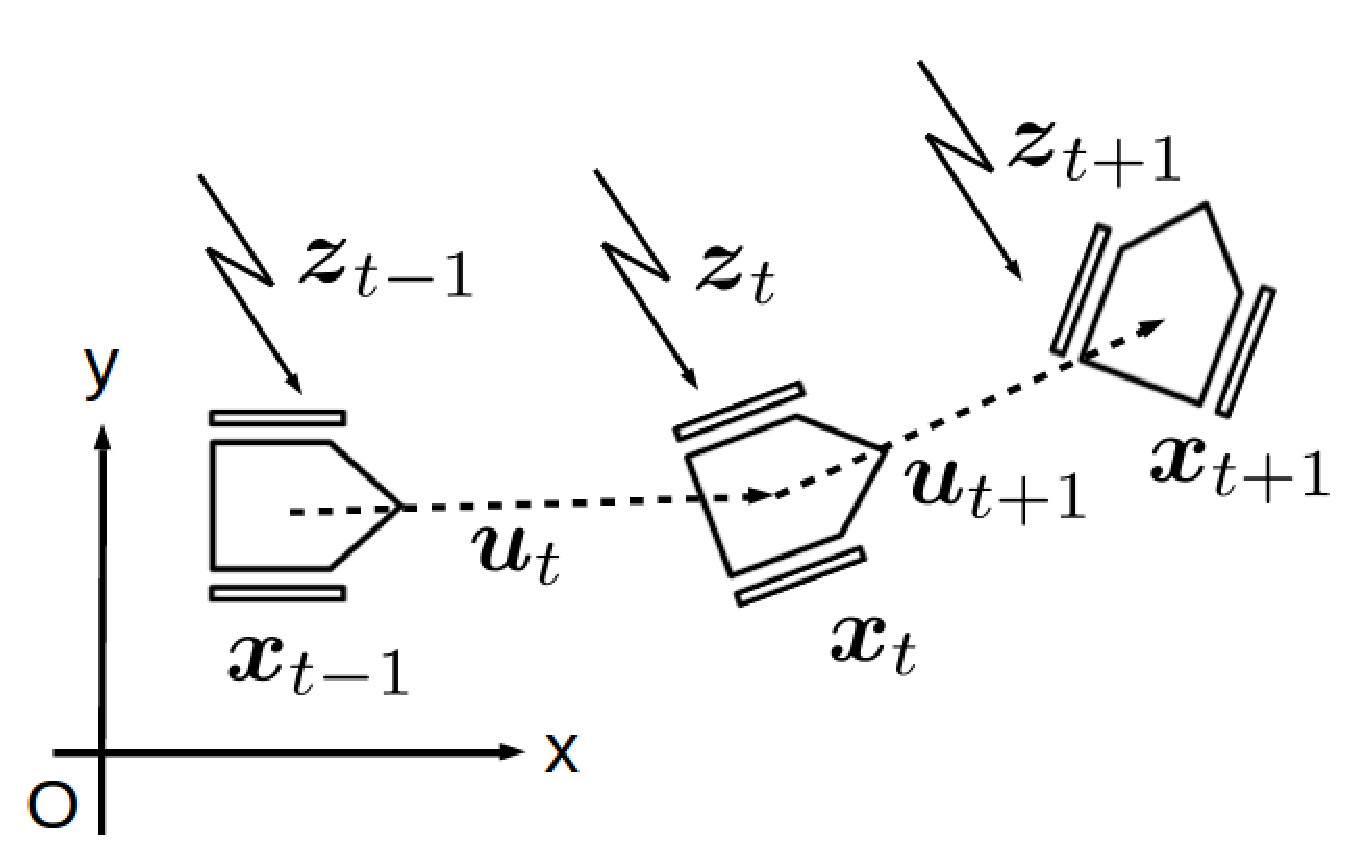
\includegraphics[width = 8cm]{./fig/symbol.eps}
    \caption{example of figure path}
    \label{fig::fig_path}
\end{figure}
